More formally, denote by \(h_{t,d}\) the number hospitalisations with
reporting date \(t\) that are known \(d\) days later. Unfortunately we
only observe \[H_{t,d} = \sum_{s = t - 6}^{t} h_{s,d + (t - s)},\]
i.e.~a weekly sum of reported hospitalisations. On day \(T\) our goal is
to predict \(H_{t,D}\) for large delays \(D\) and days \(t \leq T\), of
course it suffices to predict \(H_{t, D} - H_{t, T - t}\) and add the
known \(H_{t, T - t}\) to this prediction. We rewrite this into weekly
telescoping sum \[
H_{t,D} - H_{t,d} = \left(H_{t, d + 7} - H_{t,d}\right) + \left(H_{t, d + 14} - H_{t, d + 7}\right) + \dots + \left(H_{t,D} - H_{t, d + 7 K}\right),
\] where \(K = \lfloor (D -d) / 7 \rfloor\), reducing the task at hand
to predict hospitalisations in the \(k\)-th week ahead,
\(H_{t, d + 7k} - H_{t, d + 7\cdot(k - 1)}\), \(k = 1, \dots, K\). To
leverage known reported incidences, rewrite this as
\[\underbrace{\frac{H_{t, d + 7k} - H_{t, d + 7\cdot(k - 1)}}{I_{t,d}}}_{=:p_{t,d,k}} I_{t, d}\]
where \(I_{t,d}\) is the \(7\)-day case incidence with reporting date
\(t\) known at time \(t + d\), i.e.~the incidenct case analouge of
\(H_{t,d}\).

Assuming that the proportions \(p_{t,d,k}\) change slowly over time
\(t\) we estimate them by

\begin{align}
\label{eq:predict_p_tdk}
\widehat {p_{t,d,k}} = \frac{H_{t - 7k, d + 7k} - H_{t - 7k, d + 7\cdot(k - 1)}}{I_{t - 7k,d}} = p_{t - 7k,d,k}
\end{align}

and finally predict

\begin{align}
\label{eq:predict_H_tD}
\widehat{H_{t,D}} = H_{t,d} + I_{t,d} \left(\widehat{p_{t,d,1}} + \dots + \widehat{p_{t,d,K}}\right).
\end{align}

As hospitalisation is affected by age, we perform this procedure for all
available age groups separately and finally aggregate over all age
groups to obtain a nowcast for all age groups combined.

This describes our point nowcast for \(7\)-day hospitalisations. To
obtain uncertainty intervals we fit a normal (age groups 00-04 and
05-14) or lognormal (all other age groups) distribution to the past
performance of our model. We chose these distributions based on
explorative analysis and believe that these should be seen as heuristics
rather than as a matter of fact, which is in line with the philosophy of
our model to be as simple as possible.

Denote by \(\hat H_{t,D,s}\) the nowcast made for date \(t\) on date
\(s \geq t\). Starting with date \(t + D\) the definite \(H_{t,D}\) is
known and we can estimate the absolute prediction error
\(\varepsilon_{t,s} = H_{t,D} - \hat H_{t,D,s}\) and the relative
prediction error
\(\eta_{t,s} = \log \left( H_{t,D} - H_{t, s - t}\right) - \log \left( \hat H_{t,D,s} - H_{t, s- t} \right)\).
For the nowcast for date \(t\) made on date \(s\) we estimate the
standard deviation \(\hat\sigma\) of
\(\varepsilon_{t - D - i, s - D - i}\) or
\(\eta_{t - D - i, s - D - i}\) (age groups 00-04, 05-14 and others
respectively), \(i = 0, \dots, 27\) by its empirical counterpart. The
estimated predictive distribution which informs our prediction intervals
is then \(\mathcal N (\hat H_{t,D,s}, \sigma^2)\) (age groups 00-04 and
05-14) or
\(\mathcal{LN} \left( \log \left(\hat H_{t,D,s} - H_{t, s - t}\right), \sigma^2 \right) + H_{t, s - t}\)
(all other agr groups).

\begin{figure}
    \centering
    \includegraphics[width=\textwidth]{tikz/reporting_triangle}
    \caption{Decomposition of the daily reported hospitalisation incidences into the {\color{TUIl-orange} known incidences}, i.e. the \textbf{reporting triangle}, and {\color{TUIl-green}the future weekly increments}. {\color{TUIl-blue}The last increment} might not be a weekly one, but we expect few cases to occur for such long delays.}
    \label{fig:reporting_triangle}
\end{figure}

\subsection{Discussion}\label{subsec:nowcasting_discussion}
Before evaluating the predictive performance of our model we investigate
how the fraction of hospitalisations after one up to four weeks changes
over time across different age groups. 
\cref{fig:hospitalisation_probabilities_over_time} shows that these
fractions are changing slowely over time, especially in the older age
groups. Due to smaller numbers of infections and hospitalisations
reported in the younger age groups these fractions vary more strongly,
occassionally dropping to \(0\). Across all age groups we observe a
steady decline from October 2021 to December 2021 with a steeper drop in
fraction of hospitalisations starting with January 2022. The former
period corresponds to a time of mandatory testing at the workplace which
may improve ascertainment of asymptomatic and less severe cases. The
latter effect is most recognizable in the 35-59 age group and coincides
with the time that the Omicron variant became dominant in Germany
\citep{RobertKoch-Institut2022Lagebericht2022-01-20}. Additionally
there is no visually discernible weekday effect present in 
\cref{fig:hospitalisation_probabilities_over_time}.

\begin{figure}

    {\centering 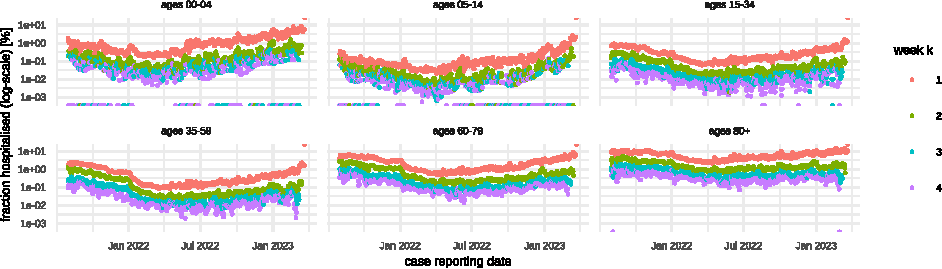
\includegraphics[width=\textwidth]{figures_tentative/hospitalisation_probabilities_over_time-1.pdf} 

}

\caption{We show the fractions of hospitalisations in the $k$-th week after case reporting date $t$  of initially reported cases in different age groups, i.e. $p_{t,0,k} = \left(H_{t,7 k} - H_{t, 7 \cdot (k - 1)}\right) / I_{t,0} $. Note the log-scale of the $y$-axis. During periods of low incidence, e.g. July -- September, we find large fluctations, but no discernable weekly pattern. With rising case numbers the fractions stabilise and decrease in most age groups. This might be due to changes in testing regime detecting less severe cases. As changes occur on slow time scales, estimating these fractions by Eq.~\eqref{eq:predict_p_tdk} is a promising approach.}\label{fig:hospitalisation_probabilities_over_time}
\end{figure}

In \cref{fig:delays_in_reporting} we depict the nowcasts produced
from our model including \(95\%\) prediction intervals, whose lengths
are based on the past performance of our model. Except for the period
from January to April 2022, the model produces reasonable nowcasts with
prediction intervals that have sensible widths. In the aforementioned
period the nowcasts overpredict the final hospitalisations, except for
the oldest age group, and, after a transitionary period, have larger
uncertainty.

\begin{figure}

    {\centering 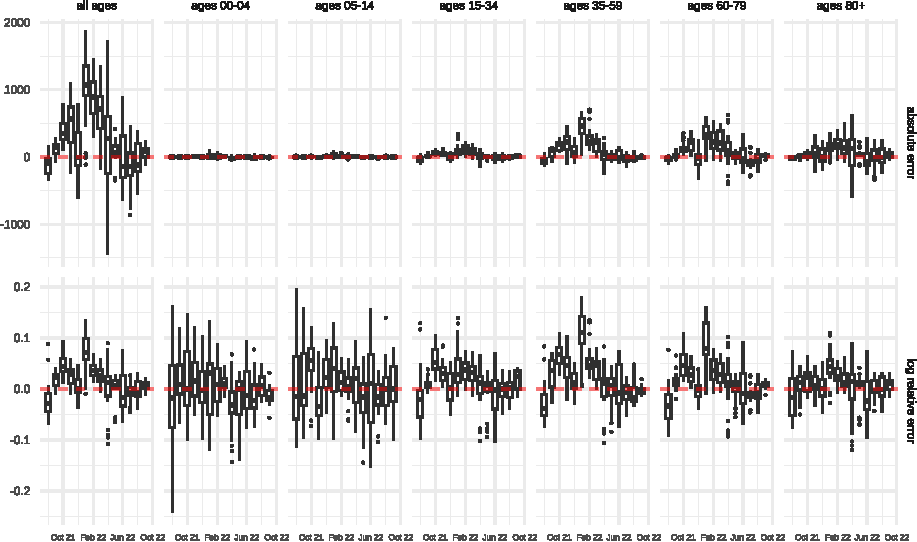
\includegraphics[width=\textwidth]{figures_tentative/REP-1.pdf} 

}

\caption{
We show relative and absolute errors of prediction of our model for same day nowcasts by month of forecast and selected age groups. 
Relative errors are displayed on the log10 scale, i.e. as $\log_{10} (\text{predicted}) - \log_{10} (\text{actual})$.
Up to December 2021 the model performs well, especially in the older age groups where most hospitalisations occur. 
The sharp increase in cases in January 2022 coupled with a lower probability of hospitalisation, most likely due to the appearance of the Omicron variant in Germany, lead to overpredictions across all age groups.
}\label{fig:REP}
\end{figure}

To investigate the quality of point predictions we display the
time-evolution of absolute (AEP) and relative errors of predictions
(REP, \(\log_{10}\)-scale) across all age groups in 
\cref{fig:REP}. From this figure one can infer that the point nowcasts
produced by our model tend to slightly overpredict the final number of
hospitalisations. Indeed, the interquartile range of REPs for all age
groups and dates combined spans \([-1.56, 8.33]\), demonstrating the
same tendency. The highest REPs occured in October / November 2021 and
January/February 2022; the first corresponding to introduction of
mandatory testing at the workplace and the second to the arrival of the
Omicron variant in Germany. In both circumstances the number of cases
rose while hospitalisations did not increase proportionally, a similar
effect to the one observed in 
\cref{fig:hospitalisation_probabilities_over_time}.

\begin{figure}

    {\centering 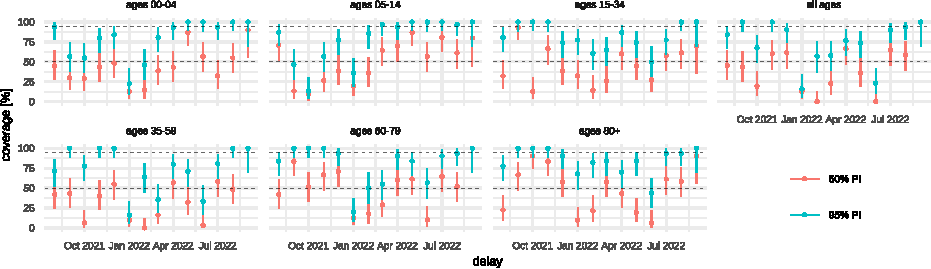
\includegraphics[width=\textwidth]{figures_tentative/coverages-1.pdf} 

}

\caption{Empirical coverage of 50\% and 95\% prediction intervals (PI) based on same-day nowcasts for dates 2021-08-01 to 2022-09-10 (406 dates) for which the true amount of hospitalisations after $12$ weeks is known as of the writing of this paper. We also display pointwise $95\%$ binomial confidence intervals for the coverage. Given the difficulties of real-time forecasting \citep{Desai2019Realtime} we deem the coverages good, except for the transitionary period in the end of 2021 where changing testing schemes and the change from Delta to Omicron cause our model to be overly confident. Coverage is generally better in the older age groups.}\label{fig:coverages}
\end{figure}

We further quantified uncertainties in estimaton by uncertainty
intervals based on an assumption of a (log)-normal distribution for the
errors with standard deviation based on past performance of our model.
In \cref{fig:coverages} we show the coverages of the \(50\%\) and
\(95\%\) prediction interval across all age groups and delays for the
whole time period of our study. For most age groups the \(50\%\)
prediction interval has close to nominal coverage, while the \(95\%\)
intervals have less than nominal coverage.

As our goal is to capture all of the uncertainty in this prediction, we
chose to assume a sensible distribution for the prediction, a normal
distribution for the two young age groups and a log-normal distribution
for all other age groups. This has the advantage of producing more
honest, wider, prediction intervals than those based on parametric
distributions. The estimated standard deviation will also account for
periods of low coverage, such as January 2022, albeit only after the
maximum delay of \(12\) weeks.

We base our choice of \(12\) weeks of delay on the empirical survival
function displayed in \cref{fig:delay_tails}. One could, however,
argue for shorter maximum delay such as \(6\) weeks because time from
reported infection to hospitalisation is much shorter, on the order of
\(\approx 10\) days \citep{Faes2020Time}, so hospitalisations after
this (shorter) period are unlikely to be due to the acute infection with
SARS-CoV-2. This would have two main benefits: The model would adapt
faster to changing circumstances and the indicator nowcasted describes
the severity of the epidemic more appropriately.

The main advantage of our model over established nowcasting approches is
its simplicity, making it easy to understand, straightforward to
implement and, once the reporting triangles for incidences and
hospitalisation are created, fast to run; taking only \(< XX\) minutes
on a standard notebook(\textbf{TODO: check!}).

The problem of nowcasting hospitalisations is different from previously
studied nowcasting settings in several ways. At the time of nowcast a
large fraction of hospitalisations are not only unobserved, but are yet
to occur - in this sense the nowcast is more accurately termed a
forecast. As the date of hospitalisation is not known, the
hospitalisations are associated by the date of reporting of the COVID-19
case, creating the double-weekday effect displayed in
\cref{fig:double_weekday_effect}. While daily updated data on
hospitalisations are available, these consist only of moving weekly
aggregates, consecutive observations are strongly auto-correlated.

We sidestep all of these issues by splitting the hospitalisations to
nowcast into weekly chunks, incorporating leading indicators of
hospitalisation -- the weekly reported case incidences -- and modelling
the number of hospitalisations to come in each chunk by binomial
thinning of incidences. Let us stress that this approach is only
possible in the special situation where case and hospitalisation are
explicitly linked, however we believe that incorporating leading
indicators into nowcasting models is a promising approach.

An additional advantage of our model is that the hospitalisation
probabilities can further be analysed, e.g.~by investigating association
between the publicly available vaccination rates and the probability of
hosptialisation and delay to hospitalisation. Sudden changes in these
fractions, as observed in 
\cref{fig:hospitalisation_probabilities_over_time}, can also hint towards
worse model performance, especially if this change can be attributed to
changing probability of hospitalisation due to new variants or changing
testing regime.

Real time forecasting of epidemiological indicators is a difficult task
\citep{Desai2019Realtime}, in particular quantifying uncertainty
\citep{Bracher2021Preregistered}. To test our model under real-time
circumstances we submitted daily nowcasts to the German COVID-19
NowcastHub \citep{2022Nowcasts} since Novemer 2021. In the nowcasting
context, \citep{Lawless1994Adjustments} goes to great lengths to
account for overdispersion due to changes in delay distribution,
introducing gamma and Dirichlet priors and explicitly modelling trends.
Such an approach would also be feasible for our approach, e.g.~model
incidences by an appropriate Poisson or negative binomial distribution
and, conditional on incidences, model hospitalisations by a binomial
distribution. As this increases the complexity of our model and relies
on the assumed distributions being sensible we opted for another
approach.

Regarding the indicator we stress that its value on a given date does
not represent the current occupancy of hospitals in Germany with
COVID-19 patients but is rather an approximation to the morbidity caused
by COVID-19 on that date. The reason for this discrepancy is that
hospitalisations are attributed to the reporting date of the associated
case, not that of hospitalisation. While the reporting date of the
hospitalisation can be recovered from the publicly available data, the
date of hospitalisation cannot. Additionally, no information on the
duration of stay is available, making it impossible to create an
indicator for the occupancy of hospitals based solely on data provided
by the \gls{rki}.

Implicit in all of these approaches is an assumption of
``stationarity'', i.e.~that future reported hospitalisations will behave
as they did in the past. Thus, all of these approaches might still be
insufficient if circumstances change drastically, for example
introduction of new testing schemes (school, 3G at workplace), changes
in the delay distribution due to new variants, or hospitals close to
capacity taking longer to process cases.

In summary, because models usually only capture a small part of the
highly dynamic data-generating process, we believe that uncertainty in
such circumstances should not come from unrealistic parametric
assumptions but rather be based on past model performance. Given the
discussed difficulties and the changing epidemiological dynamics in the
period studied, the observed errors of prediction (\cref{fig:REP})
and coverages of prediction intervals (\cref{fig:coverages}) are
satisfying.

In this paper we provide a straight-forward model for nowcasting
hospitalisations associated with COVID-19 in Germany. By leveraging
known incident cases, we can estimate fractions of hospitalisations in
weekly chunks which in turn avoids a complicated model of the two
weekday effects present in the data. As the circumstances of the
epidemic are changing constantly, e.g.~vaccination coverage, testing
regimes and emerging variants, we based uncertainty not on parametric
assumptions but on the past performance of our model, assuming a
(log)normal predictive distribution. We contributed nowcasts based on
this model since November 2021 to the German COVID-19 NowcastHub
\citep{2022Nowcasts}, a collaborative platform collecting and
aggregating such nowcasts from multiple research groups. The performance
of the nowcasts in this Hub and presented in this paper (\cref{fig:REP} and \cref{fig:coverages}) are, regarding the simplicity of
the model and the highly dynamic situation, quite satisfying.

There are multiple extensions to our model worth investigating. Firstly
hospitalisations are also available at the federal state level so
nowcasting on a spatial scale is naturally of interest due to
hetereogeneity in immunisation status and testing regimes across states.
However, splitting hospitalisations into six age groups and 16 federal
states will result in small numbers with larger variability which in
turn increases variabliity in estimates \(p_{t,d,k}\) and thus
predictions which may require some regularisation thus increasing the
models complexity. Secondly, in a similar vein, modeling the temporal
evolution of hospitalisation probabilities by smooth functions,
e.g.~splines
\citep{vandeKassteele2019Nowcasting,Schneble2021Nowcasting}, may help
in early detection of changing circumstances and thus lead to better
forecasts. Thirdly our uncertainty intervals account for the variance of
past performance, but \cref{fig:REP} suggests that there is
substantial bias in periods of changing circumstances which could be
incorporated into our model in a straightforward way. Finally to predict
the future course of the epidemic forecasting hospitalisations for dates
\(t\) that lie in the future is of interest, which could be accomplished
if one has a model that produces forecasts for incidences for all age
groups.